\chapter{Desenho da solução}

Esse capítulo tem como objetivo descrever como foi desenvolvido e desenhado a solução proposta por esse trabalho, além de apresentar resultados obtidos durante o processo.

\section{Solução proposta}

Como destacado por este trabalho anteriormente, há soluções dispostas no mercado que atendem a demanda de gestão de eventos. No entanto, foi identificado que o desenvolvimento de um aplicativo seria uma hipótese, visto os requisitos e anseios da instituição, possibilitando também demais personalizações conforme as necessidades do requisitante.

Dentre todas as citadas na Seção \ref{sec:mercado}, a que mais se aproximou do desejado foi o \textit{Doity}, porém não possui integração com sistemas terceiros, assim inviabilizando uma integração com a plataforma \textit{web} Eventos IFF. Além disso, há limitação na quantidade de participantes em eventos grátis, características as quais são essenciais.

Para a escolha da plataforma, havia como requisito características indispensáveis. A mesma deveria ser gratuita, deve apresentar uma fácil integração com a plataforma Eventos IFF, emissão de certificados e possibilidade de interação entre palestrante e inscritos, sendo assim optou-se pelo desenvolvimento de uma nova ferramenta.

\section{Diagramas da solução}

Na Figura \ref{fig:caso-de-uso} é ilustrado através do diagrama de uso as funcionalidades e ações que o usuário poderá executar no aplicativo Eventos IFF. O diagrama conta com dois atores. A audiência é o usuário que tem papel de participante do evento, já o organizador é o usuário que realiza a administração do evento, tendo acesso a todas as funcionalidades administrativas do aplicativo.

\begin{figure}[H]
    \centering
    \caption{Diagrama de caso de uso}
    \fbox{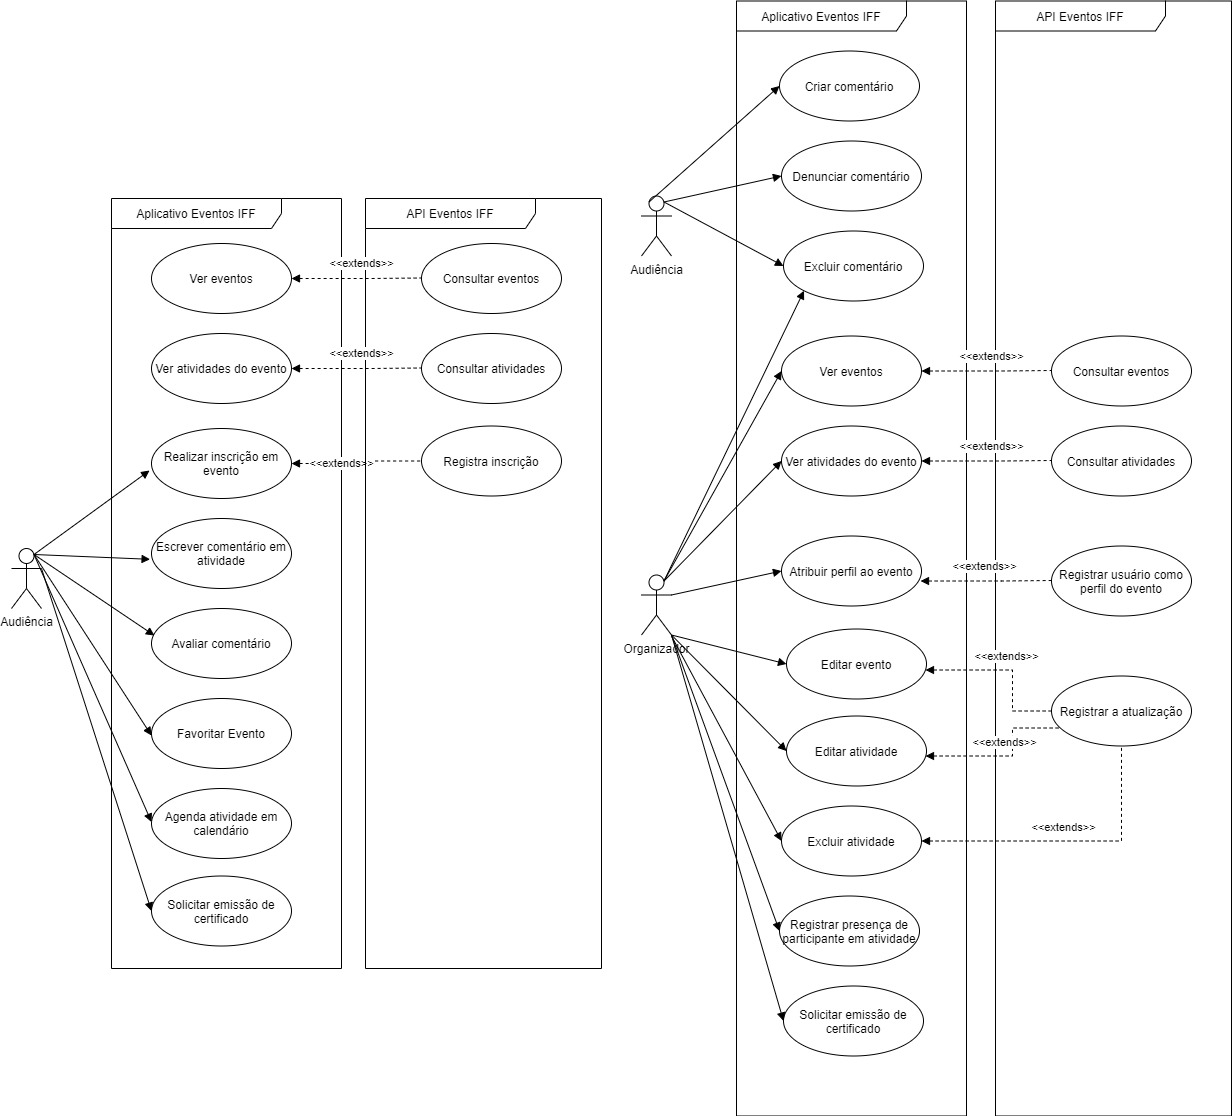
\includegraphics[scale=0.36]{figuras/caso-de-uso.jpg}}
    \label{fig:caso-de-uso}
    \legend{Fonte: elaborado pelos autores}
\end{figure}


Na Figura \ref{fig:digrama-classe} é apresentado o diagrama de classe conceitual, onde é ilustrado as principais entidades que compõem o aplicativo Eventos IFF e suas relações. Também é apresentado os 4 papeis que o usuário pode ter em relação a um evento, que são: audiência, organizador, palestrante e voluntário. Cada papel possui as funcionalidades que os usuários podem executar no aplicativo.

\begin{figure}[H]
    \centering
    \caption{Diagrama de classe conceitual}
    \fbox{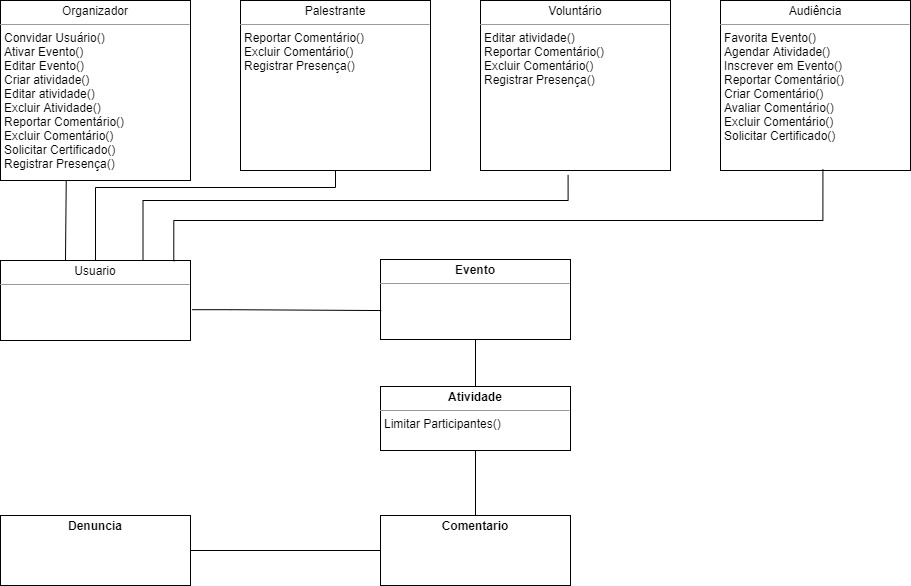
\includegraphics[scale=0.49]{figuras/diagrama-classe-conceitual.jpg}}
    % 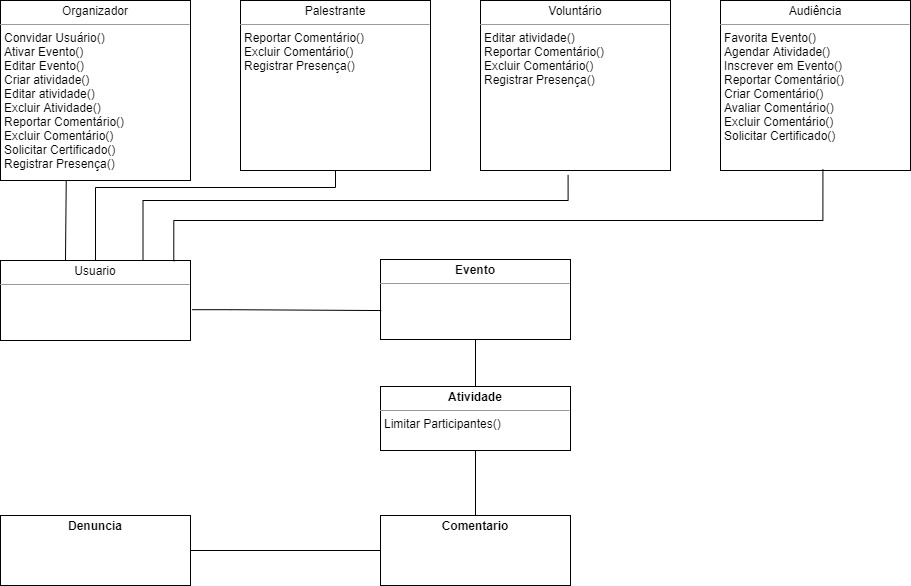
\includegraphics[scale=0.5]{figuras/diagrama-classe-conceitual.jpg}
    \label{fig:digrama-classe}
    \legend{Fonte: elaborado pelos autores}
\end{figure}

\section{Validação e execução em ambiente real}

Em novembro de 2019, no IFF Campos Centro, ocorreu o evento CITI. Ocorreram nesse evento atividades como palestras, minicursos e mesas redondas, atividades as quais necessitavam registro de presença dos participantes para geração dos certificados. Foi observado, pelos organizadores do evento, a necessidade de uma ferramenta para agilizar o registro dessas presenças. 

Diante disso, foi desenvolvido pelos os autores deste trabalho um aplicativo para dispositivos com sistema operacional \textit{Android} para atender a essa necessidade, o qual também foi utilizado para validação e estudo de parte da solução proposta deste trabalho. O aplicativo foi desenvolvido utilizando a \textit{framework} para desenvolvimento híbrido \textit{Ionic}. No entanto, foi utilizado a técnica de \textit{Minimum Viable Product} (MVP), conforme descrito por \citeonline{ries2014lean}. O objetivo foi construir um aplicativo com recursos e funcionalidades mínimas, porém viáveis, para o processo de registro de presença no evento.

Além do aplicativo, foi desenvolvida uma \textit{Application Programming Interface} (API), na linguagem PHP, que foi hospedada no servidor do IFF Campos Centro, onde possuía apenas uma rota, usando o verbo \textit{Hypertext Transfer Protocol} (HTTP) GET, para registrar a presença em um servidor \textit{Structured Query Language} (SQL). Era armazenado os seguintes dados:

\begin{itemize}
    \item CPF do participante;
    \item Nome do participante;
    \item Identificador da atividade o qual está participando;
    \item Data e hora do registro;
    \item Nome do voluntário que está realizando o registro.
\end{itemize}

O registro era feito na entrada e saída da atividade, e a informação da data e hora do registro era usada para calcular posteriormente o tempo em que o participante ficou na atividade, ajudando na validação para a geração do certificado. Além de registrar utilizando a API, também era gerado um registro dessas presenças em um arquivo \textit{Comma-Separated Values} (CSV) no dispositivo do usuário, com a finalidade de haver um \textit{backup} em caso de perdas no banco de dados.

O aplicativo era composto por duas telas. Na primeira tela, haviam dois campos, um de texto para o voluntário informar seu nome, e outro campo para o voluntário selecionar qual atividade vai ser registrada a presença. Abaixo haviam dois botões, um para prosseguir para a tela de leitura de \textit{QRCode} para registrar a presença do participante. O segundo botão abria o leitor de \textit{QRcode} do dispositivo \textit{Android} para registrar a presença de outro voluntário no dia do evento. Na Figura \ref{fig:mvp1} é apresentada esta tela.

\begin{figure}[H]
    \centering
    \caption{Tela inicial do MVP} 
    % 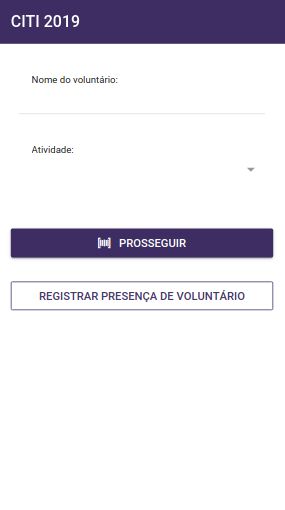
\includegraphics[scale=0.7]{figuras/mvp1.png}
    \fbox{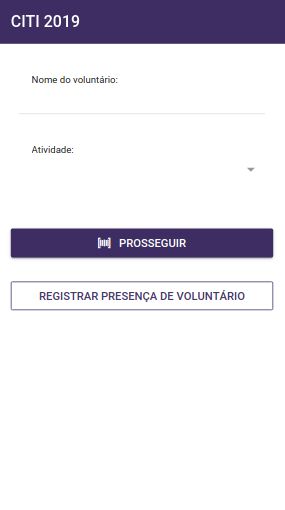
\includegraphics[scale=0.7]{figuras/mvp1.png}}
    \label{fig:mvp1}
    \legend{Fonte: elaborado pelos autores}
\end{figure}

Na segunda tela havia apenas um botão, ao qual abria o leitor de \textit{QRCode} para registrar a presença do participante (Figura \ref{fig:mvp2}). O \textit{QRCode} lido estava nos crachás de identificação dos participantes distribuídos durante o evento. No \textit{QRCode} contido nos crachás, havia a informação do nome do participante e CPF, o qual era capturado pelo aplicativo.

\begin{figure}[H]
    \centering
    \caption{Tela de leitura de \textit{QRCode} de credenciamento do MVP}
    % 
\includegraphics[scale=0.7]{figuras/mvp2.png}
    \fbox{
\includegraphics[scale=0.7]{figuras/mvp2.png}}
    \label{fig:mvp2}
    \legend{Fonte: elaborado pelos autores}
\end{figure}

\section{Análise do resultado da execução em ambiente real}

Esse MVP foi utilizado por 12 discentes que formavam parte do comitê organizador do CITI. Ao final do evento, foi produzido e distribuído pelos autores deste trabalho um questionário avaliativo, utilizando a ferramenta \textit{Google Forms}, para esses discentes. Foram obtidas 11 respostas. Esse questionário teve como finalidade saber a opinião dos usuários quanto a usabilidade e solução proposta pelo aplicativo. O questionário possuía as seguintes perguntas:

\begin{itemize}
    \item A tela de credenciamento é intuitiva?
    \item A tela de leitura do \textit{QRCode} é intuitiva?
    \item De modo geral a aplicação foi de fácil utilização?
    \item O arquivo de \textit{backup} local foi de fácil acesso?
    \item Aplicação apresentou algum tipo de falha?
    \item Caso apresentou falha, descreva.
    \item Sugestões de melhorias.
\end{itemize}

Com as respostas obtidas pelo formulário, foi observado que o \textit{layout} das telas foram bem aceito, com 100\% das respostas indicando que eram intuitivas e de fácil utilização. Não foi indicado nenhuma falha na utilização do aplicativo. Como sugestões, foi informado uma melhoria na funcionalidade de \textit{backup} e colocar mais imagens no aplicativo. O formulário utilizado para a pesquisa de opinião está disponível no Apêndice \ref{apendice1}, assim como o resultado obtido pelo formulário, onde se encontra no Apêndice \ref{apendice2}.

\section{Desenho da estrutura e funcionalidades}

Após análise dos resultados obtidos com a utilização do aplicativo para credenciamento no CITI, foi iniciado a análise da plataforma Eventos IFF, onde foi avaliado as suas funcionalidades e quais funcionalidades poderiam ser acrescentadas com uma aplicação móvel, baseado na experiência obtida no CITI. Foram feitos levantamentos de requisitos para entendimento melhor da plataforma. 

Ao finalizar essa etapa, foi desenhado \textit{wireframes} ilustrando as funcionalidades vistas inicialmente como relevantes para o aplicativo. Na Figura \ref{fig:wireframe1} e \ref{fig:wireframe2} é mostrado dois \textit{wireframes} desenvolvidos nessa etapa, o primeiro ilustrando a página principal do aplicativo e o segundo com a primeira estrutura idealizada para a funcionalidade de envio de perguntas para o palestrante.

% \begin{figure}[H]
%   \begin{minipage}[b]{0.4\textwidth}
%     \caption{Wireframe da tela inicial do aplicativo}
%     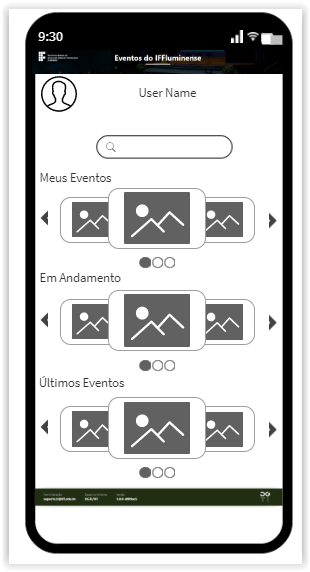
\includegraphics[width=\textwidth]{figuras/wireframe1.PNG}
%     \label{fig:wireframe1}
%     \legend{Fonte: elaborado pelos autores}
%   \end{minipage}
%   \hfill
%   \begin{minipage}[b]{0.4\textwidth}
%     \caption{Wireframe da tela de envio de comentários em atividade}
%     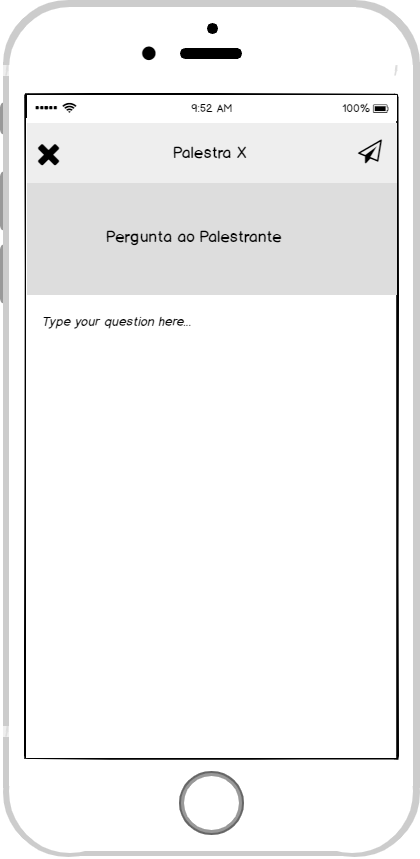
\includegraphics[scale=0.37]{figuras/wireframe2.png}
%     \label{fig:wireframe2}
%     \legend{Fonte: elaborado pelos autores}
%   \end{minipage}
% \end{figure}

\begin{figure}[H]
    \centering
    \caption{\textit{Wireframe} da tela inicial do aplicativo}
    % 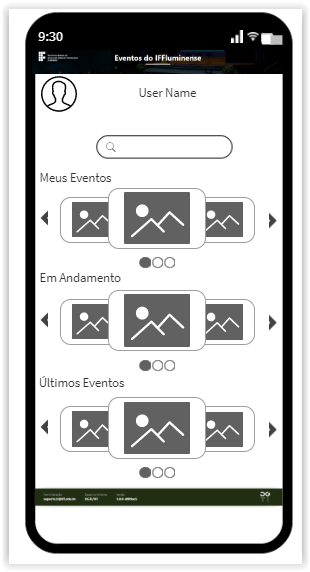
\includegraphics[scale=0.81]{figuras/wireframe1.PNG}
    \fbox{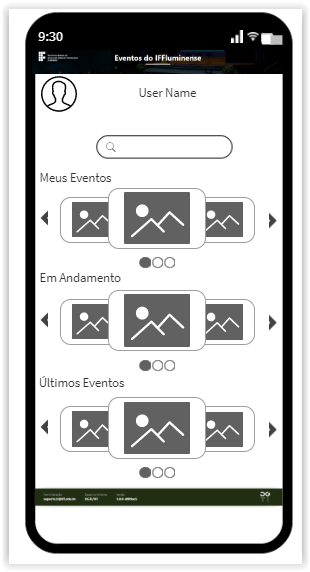
\includegraphics[scale=0.81]{figuras/wireframe1.PNG}}
    \label{fig:wireframe1}
    \legend{Fonte: elaborado pelos autores}
\end{figure}

\begin{figure}[H]
    \centering
    \caption{\textit{Wireframe} da tela de envio de comentários em atividade}
    % 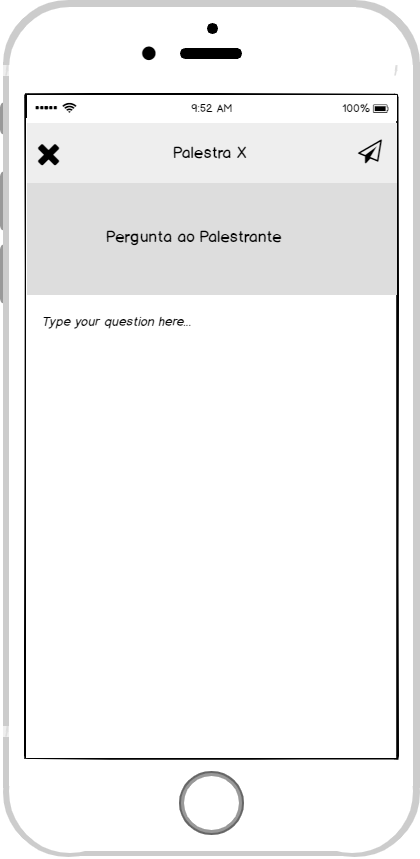
\includegraphics[scale=0.4]{figuras/wireframe2.png}
    \fbox{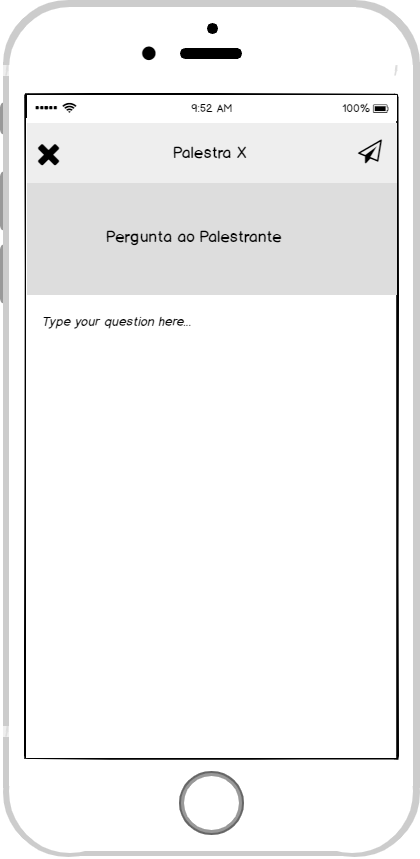
\includegraphics[scale=0.4]{figuras/wireframe2.png}}
    \label{fig:wireframe2}
    \legend{Fonte: elaborado pelos autores}
\end{figure}

Com a definição das funcionalidades e requisitos, foram desenvolvidos os diagramas de caso de uso e de classe. Com esses diagramas, alguns impedimentos e correções nas funcionalidades inicialmente pensadas ficaram mais esclarecidas, o que foram corrigidas com novas revisões nos requisitos levantados e correções nos diagramas. Em seguida foi desenhada a arquitetura dessa solução, visando ilustrar como seria a comunicação entre os serviços do Eventos IFF com o \textit{website} Eventos IFF e o aplicativo proposto por esse trabalho, além da comunicação com a plataforma \textit{Firebase}.

Nas Figuras \ref{fig:classe} é apresentado o diagrama de classe da aplicação. Na Figura \ref{fig:arquitetura} é ilustrada a arquitetura da integração do aplicativo com os serviços do Eventos IFF, assim como com o \textit{Firebase}.

\begin{figure}[H]
    \centering
    \caption{Diagrama de classe}
    % 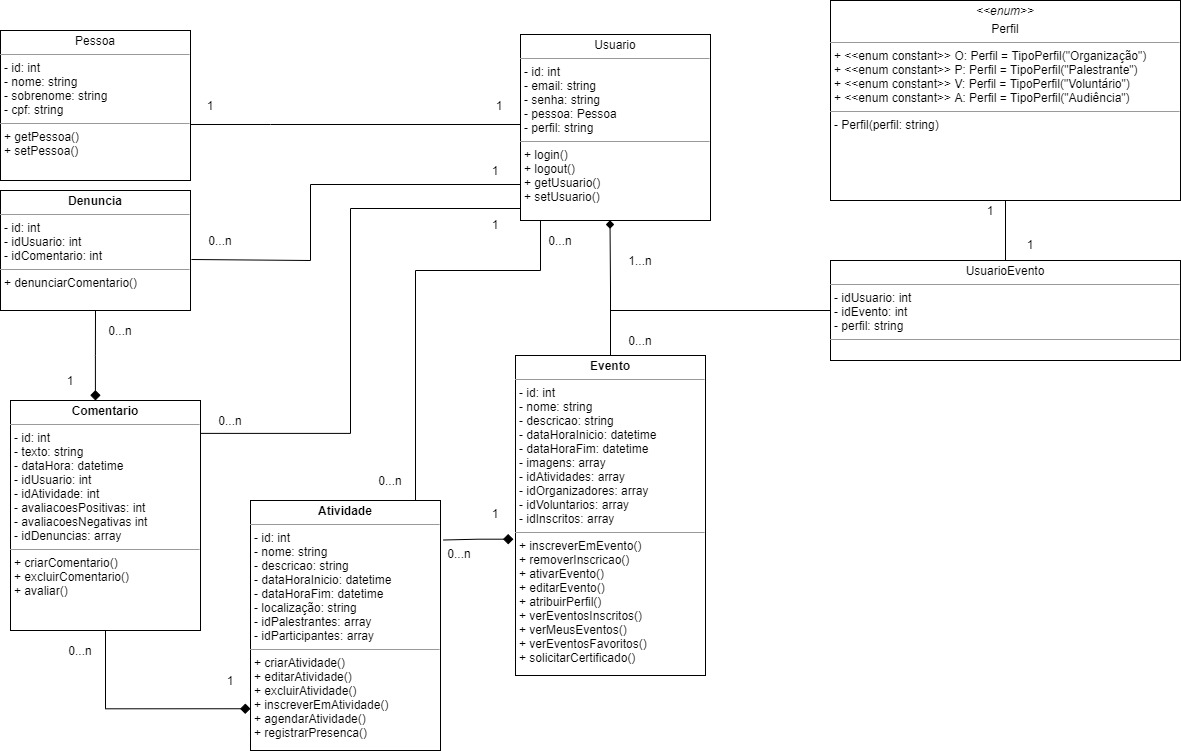
\includegraphics[scale=0.4]{figuras/Diagrama-de-classe.jpg}
    \fbox{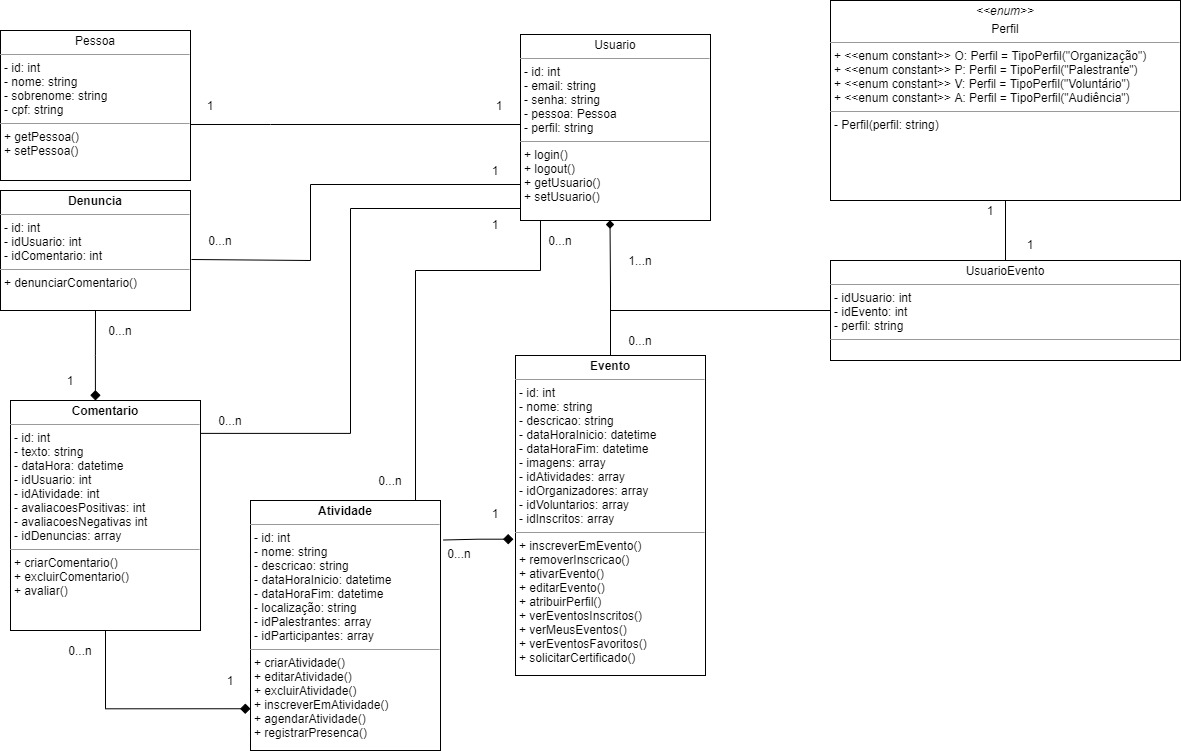
\includegraphics[scale=0.365]{figuras/Diagrama-de-classe.jpg}}
    \label{fig:classe}
    \legend{Fonte: elaborado pelos autores}
\end{figure}

\begin{figure}[H]
    \centering
    \caption{Arquitetura da integração do aplicativo com o Eventos IFF}
    % 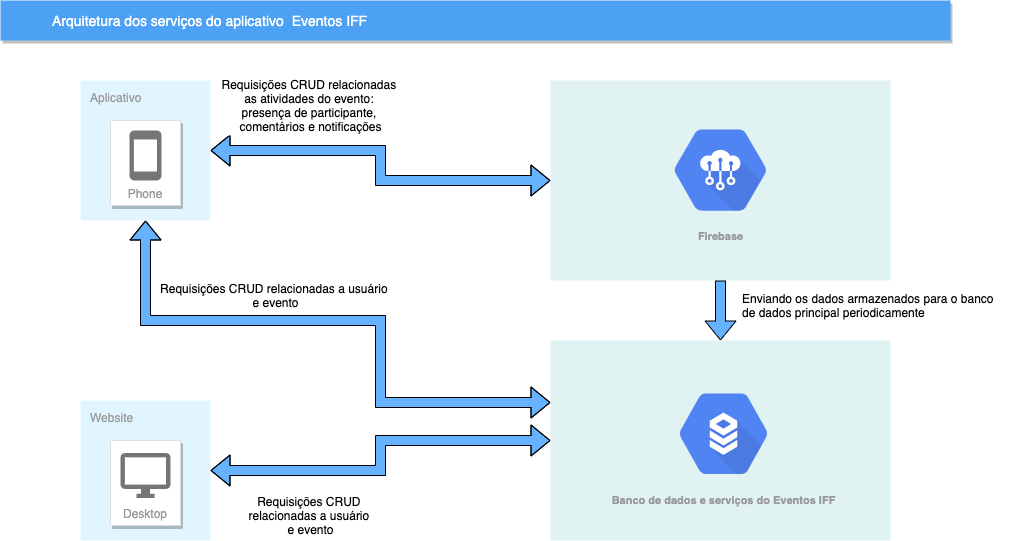
\includegraphics[scale=0.475]{figuras/Arquitetura.png}
    \fbox{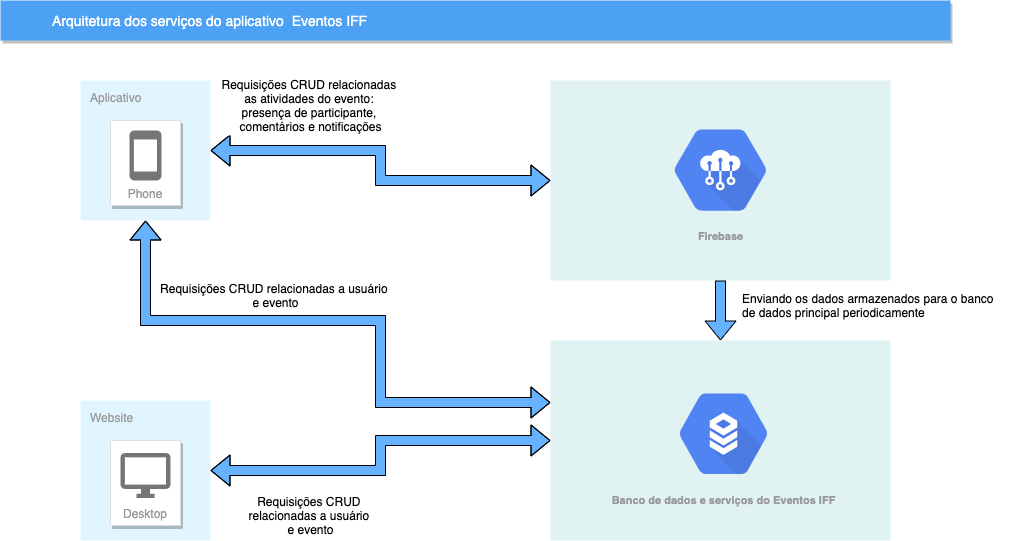
\includegraphics[scale=0.445]{figuras/Arquitetura.png}}
    \label{fig:arquitetura}
    \legend{Fonte: elaborado pelos autores}
\end{figure}

\subsection{Uso do \textit{Firebase} na arquitetura}

O \textit{Firebase} possui uma ferramenta, no qual é chamada de \textit{Firestore Database} ou \textit{Cloud Firestore}, onde consiste em um banco de dados não relacional, flexível e escalonável, que é indicado para desenvolvimento de dispositivos móveis, além de aplicações \textit{web} \cite{google_firebase}.

O \textit{Firestore Database} oferece uma sincronia em tempo real entre o dispositivo cliente e o banco de dados. Isso é possível através de ouvintes que atuam no dispositivo cliente através da integração com o \textit{Firestore Database}, onde atualiza os dados no dispositivo cliente logo após sua mudança no banco de dados \cite{google_firebase}. Na Figura \ref{fig:firebase} é exibido um exemplo da estrutura de armazenamento do \textit{Firestore Database} na interface do \textit{Firebase}.

\begin{figure}[H]
    \centering
    \caption{Interface do \textit{Firestore Database} no \textit{Firebase}}
    % 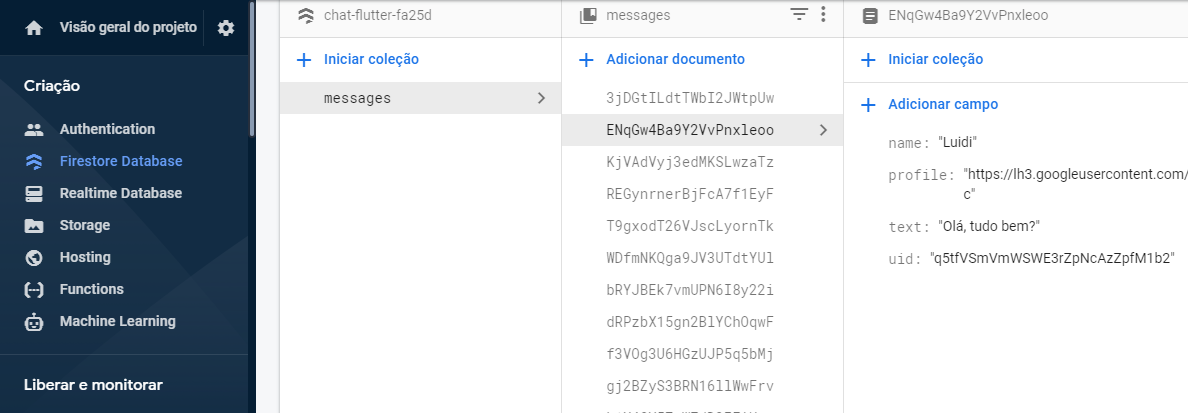
\includegraphics[scale=0.5]{figuras/firebase.PNG}
    \fbox{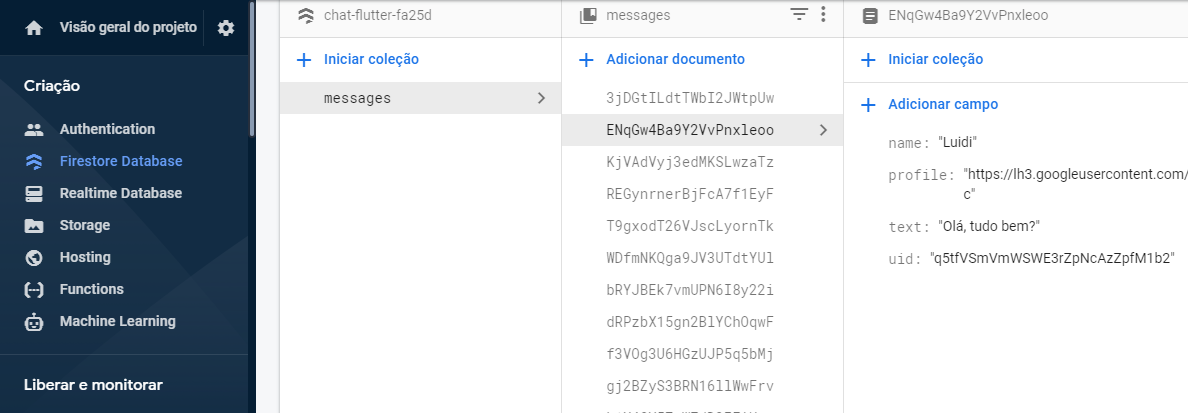
\includegraphics[scale=0.503]{figuras/firebase.PNG}}
    \label{fig:firebase}
    \legend{Fonte: \textit{website} do \textit{Firebase}}
\end{figure}

Deste modo, para a funcionalidade de comentários na atividade do aplicativo Eventos IFF, essa sincronia em tempo real do \textit{Firestore Database} se torna fundamental para uma boa experiência do usuário, onde os novos comentários feitos por outros usuários na atividade são exibidos em tempo real para o usuário que estiver visualizando essa tela.